\chapter{Theoretische Grundlagen}
%NOTES:
%-> verteilte systeme zeug
 %   -> sync and async data exchange
  %  -> verschlüsselung
   % -> Authentifizierung
 %   -> Business Data Objects (BDO)
%    -> 
%websockets
%opcua
%knoten und kanten
%datenbanken
%was ist eine db?
%-> normalformen
%-> referenzielle integrität
%-> sql
%webdevelopment
%-> js frameworks
%-> vue
%-> JSON
%-> XML
%-> REST
%interfaces
%->general
%->impl. in JS
%->impl. in C++
\section{SCADA}
\section{Verteilte Systeme}
\subsection{Synchrones Datenmodell}
\subsection{Asynchrones Datenmodell}
\section{Security}
\subsection{Authentifizierung}
\subsection{Verschlüsselung}
\section{Safety}
\section{Websocket}

\section{Datenbanken}
\subsection{Relationale Datenbank}\label{subsec:relDB}

Unter einer Datenbank versteht man einen Server der Tabellen mit Datensätzen speichert und im Netzwerk zur Verfügung stellt.
Eine Datenbank ermöglicht den schnellen Zugriff auf Datensätze und ermöglicht die Verknüpfung dieser Daten. Jeder Datensatz in einer Tabelle muss eindeutig durch einen Primärschlüssel (primaryKey) zu erreichen sein. Dieser Schlüssel kann aus einer oder mehreren Spalten einer Tabelle definiert werden. Außerdem bietet die Datenbank die Möglichkeit, weitere Schlüssel sogenannte \emph{unique Keys}, zu definieren welche wieder einzigartig für jeden Datensatz innerhalb einer Tabelle sein müssen.\\
Die dritte Art von Key, ist der \emph{foreignKey}.\\
Dieser Key wird nicht von jeder Datenbankengine unterstützt und ermöglicht die Beschreibung von Relationen, direkt in der Datenbank. 
So Kann man zum Beispiel eine Tabelle mit Risiken (\emph{RiskRisks}) haben, sowie eine Tabelle mit Lebensphasen des Produkts (\emph{RiskLifephases}). Jede Tabelle enthält als Primärschlüssel eine Spalte des Typs \emph{unsigned int} mit dem Namen \emph{ID}. Außerdem enthalten sie Spalten, die Informationen zu den Lebensphasen und Risiken beschreiben.
Eine dritte Tabelle (\emph{RiskDocument}) repräsentiert die fertigen Dokumente. Sie einhält wieder einen ID Spalte als Primärschlüssel sowie eine ComponentID, RiskID sowie LifephaseID Spalte. Letztere sind sind vom selben Typ (\emph{unsigned int})wie die Primärschlüssel der Tabellen \emph{Components} (im Releasemanagement), \emph{RiskRisks} sowie \emph{RiskLifephases}. Dies ermöglicht es, diese Spalten jeweils als foreignKey auf die jeweiligen Tabellen zu definieren und somit die Relation ausreichend zu beschreiben, sodass die Datenbank nun selbständig ihre Integrietät hält. Genau dieses Verhalten wünscht man sich von einer relationalen Datenbank.
Wenn man zum Beispiel versuchen würde eine Lebensphase zu löschen, prüft die Datenbank zuerst, ob nicht eine andere Tabelle, die einen foreignKey auf die Lebensphasen Tabelle hält (zum Beispiel die Tabelle \emph{RiskDocument}), einen Datensatz beinhaltet welcher eine Referenz auf die zu löschende Lebensphase darstellt. Wenn dies zutreffen würde, gäbe es 2 Möglichkeiten wie die Datenbank darauf reagieren könnte.
\begin{itemize}
	\item Die Datenbank löscht die Lebensphase nicht und reagiert auf die Anfrage mit einer Fehlermeldung
	\item Die Datenbank löscht alle Datensätze die auf die zu löschende Lebensphase referenzieren
\end{itemize}
Welche dieser 2 Aktionen ausgeführt werden, kann man beim Erstellen des foreignKey definieren. Jedoch bleibt in beiden Fällen die Integrietät erhalten und es gibt danach keine Referenzen auf Datensätze die nicht mehr existieren.
%was ist eine relationale datenbank?
%warum nutzt man eine relational datenbank?
\subsection{\acs{sql}}
\acs{sql} ist eine Abkürzung für \acl{sql}. Dabei handelt es sich um eine Sprache, welche das Erzeugen und Verwalten von Datenstrukturen ermöglicht. Außerdem ermöglicht sie das Abfragen, Einfügen, Verändern, sowie Verknüpfen von Datensätzen.
Dabei unterscheidet sich SQL sehr von anderen Programmiersprachen.
So besteht der Ansatz bei SQL eher darin, dass man eher definiert was man gerne als Erbegnis hätte, sich aber um die konkrete Implementierung der Operation, keinerlei Gedanken machen braucht.
Um dies zu demonstrieren ist das folgende einfache Beispiel gegeben.
\begin{figure}[hbt]
  	\centering
    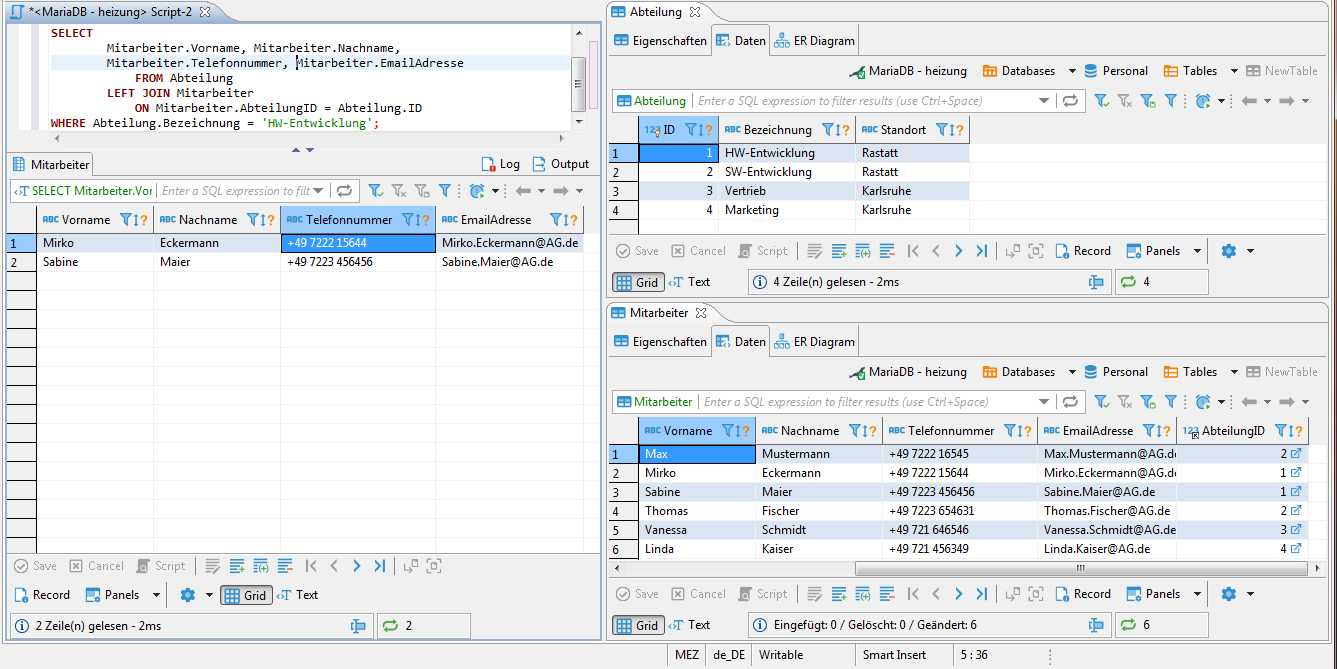
\includegraphics[width=\textwidth]{content/hauptteil/theoretischeGrundlagen/rec/exampleSQL.png}
	\caption{Beispiel Datenstruktur}
 	\label{fig:exampleSQLStructure}
\end{figure}
\begin{figure}[hbt]
  	\centering
    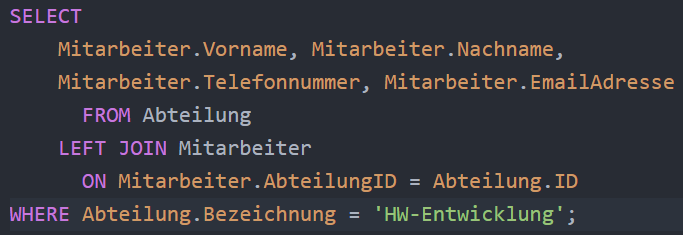
\includegraphics[width=\textwidth]{content/hauptteil/theoretischeGrundlagen/rec/sqlQuery.png}
	\caption{Beispiel sqlQuery - Select mit Join}
 	\label{fig:exampleSQLQuery}
\end{figure}
Wie in Abbildung \ref{fig:exampleSQLStructure} zu sehen, besteht die Datenbank \emph{Personal} aus zwei Tabellen.
Die erste Tabelle (\emph{Abteilung}) mit den Spalten \emph{ID}, \emph{Bezeichnung} sowie Standort.
Die Spalte \emph{ID} ist als primaryKey deklariert.
Die zweite Tabelle (\emph{Mitarbeiter}) mit den Spalten \emph{Personalnummer}, \emph{Vorname}, \emph{Nachname}, \emph{Telefonnummer}, \emph{EmailAdresse}, \emph{AbteilungID}.
Nun möchte man gerne alle Telefonnummern, Namen und E-mail Adressen einer Abteilung haben, welche den Namen \emph{HW-Entwicklung trägt}.
Der Query dafür ist in Abbildung \ref{fig:exampleSQLQuery} abgebildet.
Die Antwort des Servers ist in Abbildung \ref{fig:exampleSQLStructure} unten links zu sehen.
Rechts seht  man die beiden Quelltabellen des Queries.
Wahrscheinlich würde man diesen einfachen Datenbank Join, in C/C++, mit den Daten in Structures gespeichert, mittels verschachtelter For-Schleifen implementieren. Dass Problem bei dieser Implementierung ist, man muss durch jedes Element itterieren.
Die Datenbank hat zur Lösung dieses Problems bessere Algorithmen hinterlegt (Stichwort Binärer Suchbaum).
Außerdem hat man mit einem Sql-Server als Backend den Vorteil, dass die Applikation ohne weiteren Aufwand auch Multiuserended sein kann ohne wirklich mehr Code zu schreiben.
%was ist SQL
%was sind vor/nachteile von SQL (wann ist sql performant)
%Verknüpfung von daten(google facebook (sie waren doch dieser, der ... ))
\subsection{Stored Procedurs}\label{subsec:storedProc}
%Was sind Stored Procedurs
%warum wurden sie speziel in Green eingesetzt
Ein Sql-Server unterstützt nicht nur das Manipulieren von Daten durch eine Client-Anwendung, sondern auch das Speichern von Funktionen und Prozeduren, welche in SQL geschrieben sind.
Der wesentliche Unterschied zwischen einer Prozedur und einer Funktion besteht darin, dass eine Funktion einen Rückgabewert haben kann, eine Prozedur dagegen nicht.
Das Fehlen eines Rückgabewerts einer Prozedur stellt aber, entgegen der allgemeinen Erwartung, kein Handicap dar. Prozeduren und Funktionen akzeptieren nähmlich auch sessionbezogene globale Variablen als \emph{OUT} Argument. 
Desweiteren haben Prozeduren entgegen Funktionen die Möglichkeit, SQL-Queries zur Laufzeit zusammenzusetzen und auszuführen.

\section{Echtzeitfähigkeit}
\section{OPCUA}